\documentclass[10pt]{article}
\usepackage{longtable}
\usepackage{graphicx}
\usepackage{threeparttablex}
\usepackage{threeparttable}
\usepackage{lscape}
\usepackage{comment}

\setlength{\topmargin}{0.0cm}
\setlength{\textheight}{21.5cm}
\setlength{\oddsidemargin}{0cm} 
\setlength{\textwidth}{16.5cm}
\setlength{\columnsep}{0.6cm}

\newcommand{\version}{2.0.8 }
\newcommand{\iSGcurrent}{indel-seq-gen-\version }
\newcommand{\iSGcurrentshort}{iSGv\version }
\newcommand{\iSGcurrentlong}{indel-Seq-Gen v\version }

%%%%%%%%%% 
%%% When defining a comment, note that the \begin{GUI} MUST be
%%%  (i) on a line of its own, and
%%%  (ii) be flush left (not even spaces before it.
%%%%%%%%%% 

\begin{document}

\excludecomment{GUI}
\excludecomment{GUI2}
\excludecomment{GUI3}

\title{\iSGcurrentlong Manual}
\author{Cory L. Strope\thanks{Corresponding Author, University of Nebraska, email: 
        corystrope@gmail.com}, Computer Science and Engineering,\\
        Kevin Abel, Computer Science and Engineering,\\
        Stephen D. Scott, Computer Science and Engineering,\\
        Etsuko N. Moriyama, School of Biological Sciences and the Center for Plant Science Innovation\\~\\
		University of Nebraska -- Lincoln
}

\maketitle

\tableofcontents
\newpage
\section{Acknowledgments}

We would like to thank the authors of Seq-Gen, Drs. Andrew Rambaut and Nick Grassly, which provided the starting point for the development of iSG. As such, when citing indel-Seq-Gen, please note that Seq-Gen~\cite{Rambaut97} should also be cited. The bibtex citation is:

\begin{verbatim}

@ARTICLE{Rambaut97,
        AUTHOR = "A. Rambaut and N.C. Grassly",
        TITLE = "{Seq-Gen}: an application for the {Monte Carlo} simulation of 
{DNA} sequence evolution along phylogenetic trees",
        JOURNAL = "{CABIOS}",
        VOLUME = 13,
        NUMBER = 3,
        YEAR = 1997,
        PAGES = "235-238"       }

\end{verbatim}

We are also grateful for the NSF AToL grant 0732863 and Department of Education grant P200A040150 for funding this work.

\newpage

\section{Introduction}

indel-Seq-Gen is a tool to simulate the evolutionary events of highly diverged DNA (coding and non-coding) and protein sequences.  Long-term evolution often include dynamic changes such as insertions and deletions (indels), but some subsequences, such as domains and
motifs, retain their original sequences and structures better than less functionally important regions.  indel-Seq-Gen allows for the simulation of many different evolutionary patterns over different regions of a sequence, in the end outputting the ``true'' multiple alignment of the sequences.  indel-Seq-Gen also has multiple unique features, including input a multiple alignment for the root sequence\footnote{This can be used to create different but related ancestral sequences in each run}, placing functional constraints on sequence sites, tracing mutations along the simulation and noting their positions in the true multiple alignment, changing evolution parameters and site conservation between subtrees (i.e., lineages), and more. In addition \iSGcurrentshort fixes a fundamental flaw in representing in representing insertions and deletions through the introduction of evolving along the guide tree in discrete steps. Finally, \iSGcurrentshort also introduces a novel method of representing conservation patterns with respect to insertions versus deletions versus substitutions. These features can be used in many evolutionary studies, such as to test the accuracy of multiple alignment methods, phylogenetic methods, evolutionary hypotheses, ancestral sequence reconstruction methods, and superfamily classification methods.

\section{Getting Started}

\iSGcurrentlong (\iSGcurrentshort) is freely downloadable at {\tt http://bioinfolab.unl.edu/$\sim$cstrope/iSG/}. \iSGcurrentshort has been tested MacOS X (versions 10.4.7 and Leopard).  You will need {\tt g++} compiler if the provided executables do not run on your system.

\begin{enumerate}
\item Download the {\tt \iSGcurrent.tar.gz} source archive, open the archive by typing the two commands:
 \begin{itemize}
 \item[] {\tt gunzip \iSGcurrent.tar.gz}, and then
 \item[] {\tt tar -xvf \iSGcurrent.tar}
 \end{itemize}
\item This creates a directory {\tt \iSGcurrent} with all of the files.  Go to this directory {\tt cd \iSGcurrent}. Make the executables of indel-seq-gen by typing the command ``{\tt ./configure}'', followed by the command ``{\tt make}''. For further installation instructions, refer to the file {\tt INSTALL}. 
\item After making the executables, type the command ``{\tt cp src/indel-seq-gen data/}''. This copies the executable into the {\tt data} directory.
\item Go to the {\tt data} directory using the command ``{\tt cd data/}''.
\item In the {\tt data} directory, there are sample files that can be used to run indel-seq-gen. The following commands will execute indel-seq-gen using various capabilities. Cut-and-paste (or type) these examples to run the simulations. After each run, you can examine the output of these runs by opening the filenames that begin with the name following the {\tt --outfile} or {\tt -e} flags:
\begin{verbatim}
./indel-seq-gen --matrix HKY --outfile DNA_out < simple_nuc.tree
./indel-seq-gen --matrix HKY --codon_rates 0.2,0.05,0.75 --outfile DNA_out < simple_nuc.tree
./indel-seq-gen -m HKY -e mid_noncoding --num_runs 5 < mid_nuc_noncoding.tree
./indel-seq-gen -m HKY -e mid_noncoding -n 5 -c 2,1,8 --invar 0.02 < mid_nuc_coding.tree
./indel-seq-gen -m HKY -c 2,1,8 -e exon_intron --step_type trs < exon_intron.tree
./indel-seq-gen -m HKY -c 2,1,8 --lineage exon_intron_lineage.spec < exon_intron_lineage.tree
./indel-seq-gen -m JTT -k lipocalin.spec -w a  --alpha 1.3 < lipocalin.tree
./indel-seq-gen -m JTT -k lipocalin_ma.spec < lipocalin_ma.tree
\end{verbatim}
 For further understanding of these examples, refer to Section~\ref{sec:example}.

\begin{GUI}
\item The {\tt \iSGcurrent/data} directory is the default working directory for the GUI interface for \iSGcurrentshort. Refer to Section~\ref{sec:GUI} for instructions on changing the default working directory. This working directory should contain the data files needed for the simulation. A script file, {\tt isgRemote}, is generated by the GUI interface to run iSGcurrentshort will also be created in this directory.
\end{GUI}
\end{enumerate}


%%%%%%%%%%
%%% NEW SECTION: ISGVXX PARAMETERS
%%%%%%%%%%
\section{Overview}
\label{sec:overview}

In order to simulate heterogeneous sequences and lineage- and site-specific \iSGcurrentshort uses \textit{enviroments}. The environment of simulation is comprised of
substitution parameters ($\Theta$; four components: $\theta^m \rightarrow$ substitution matrix , $\theta^f \rightarrow$ character frequencies, $\theta^r \rightarrow$ site rates, and $\theta^i\rightarrow$ percent invariable sites) and indel parameters ($\Lambda$; three components: $\lambda^p \rightarrow$ probability of an indel occurring as the number of indels per subsitution, $\lambda^l\rightarrow$ length distribution, and $\lambda^m\rightarrow$ maximum length). \iSGcurrentshort implements four environments: 

\begin{enumerate}
\item \textit{Global environment}: Sets the default substitution parameters for the simulation run (indel parameters cannot be specified globally).
\item \textit{Partition environment}: Defines the partition-specific simulation parameters.
\item \textit{Subtree environment}: Defines the lineage-specific simulation parameters.
\item \textit{Motif environment}: Defines site-specific simulation parameters.
\end{enumerate}

Besides the motif environment, these environments define the same sets of parameters. For this reason, \iSGcurrentshort implements precedence for each variable, where the precedence, from lowest to highest, is global, partition, subtree. If any components of the substitution or indel parameter ar not changed in a higher precedence environment, that component inherits the settings from the next lower precedence environment. The motif environment does not conflict with the substitution and indel settings of the other environments, as it works specifically on sites. Precedence and settings can be found in Table~\ref{tab:precedence}, and an example simulation run using the precedence rules is shown in Figure~\ref{fig:simulation_run}.

\begin{center}
\begin{threeparttable}
\caption{\it Listing of the precedences of environments and the sections in hich environments are explained.}
\begin{tabular}{lllll}
\hline\hline
            &        & \multicolumn{2}{c}{Precedence} & \\\cline{3-4} 
Environment & Set in   & $\Theta$\tnote{1} & $\Lambda$\tnote{1} & Section 
\\\hline
Global    & Command line       & Low      & N/A & \ref{sec:global_options} \\
Partition & Guide tree file    & Middle   & Low & \ref{sec:partition_options}\\ 
Subtree   & Specification file & High     & High&\ref{sec:lineage_options} \\
Motif     & Specification file & N/A      & N/A &\ref{sec:motif_options} \\
\hline\hline
\end{tabular}
\begin{tablenotes}
\item[1] $\Theta = \{\theta^m,\theta^f,\theta^r,\theta^i\}$ are the substitution parameters, as defined in Section~\ref{sec:overview}.
\item[2] $\Lambda = \{\lambda^p,\lambda^l,\lambda^m\}$ are the indel parameters, as defined in Section~\ref{sec:overview}.
\end{tablenotes}
\label{tab:precedence}
\end{threeparttable}
\end{center}

Table~\ref{tab:precedence_specific} gives the precedence overriding options for each of the environments.

\begin{center}
\begin{threeparttable}
\caption{\it Environment options and the options that override them for the different input files to \iSGcurrentshort.}
\begin{tabular}{cclll}
 \hline \hline
 && \multicolumn{3}{c}{Lowest $\longleftarrow$ Precedence $\longrightarrow$ Highest} \\\cline{3-5}
 && \multicolumn{1}{c}{Global\tnote{1}} & \multicolumn{1}{c}{Subtree\tnote{2}} & \multicolumn{1}{c}{Lineage\tnote{3}} \\
\hline
 
 $\Theta$:
 & $\theta^f$ 
   & \texttt{-f (--frequencies) $<$float\_list$>$}
   & \texttt{\#$<$filename$>$\# }
   & \texttt{\#f$<$filename$>$\#}
 \\\\
 & $\theta^m$ 
   & \texttt{-m (--matrix) $<$matrix$>$}
   & \texttt{\#m$<$matrix$>$\#}
   & \texttt{\#m$<$matrix$>$\#}
 \\\\
 & $\theta^r$ 
   & \texttt{-g (--num\_gamma\_cats) $<$int$>$}
   & \texttt{\#r\#} 
   & \texttt{\#r\#} {\small OR}
 \\
 & 
   &
   &
   & \texttt{\#g$<$int$>$\#}
 \\
 & 
   & \texttt{-a (--alpha) $<$float$>$}
   & \texttt{\#r\#}
   & \texttt{\#r\#} {\small OR}
 \\
 &
   &
   &
   & \texttt{\#a$<$float$>$\#}
 \\
 &
   & \texttt{-c (--codon\_rates) $<$float\_list$>$}
   & \texttt{\#r\#}
   & \texttt{\#r\#} {\small OR}
 \\
 &
   &
   &
   & \texttt{\#c$<$float\_list$>$\#}
 \\\\
 & $\theta^i$ 
   & \texttt{-i (--invariable) $<$float$>$}
   & \texttt{\#r\#} {\small OR}
   & \texttt{\#r\#} {\small OR}
 \\
 &
   &
   & \texttt{\#i$<$float$>$\#}
   & \texttt{\#i$<$float$>$\#}
 \\
 \hline
 $\Lambda$\tnote{4}:
 & $\lambda^m$
   & \multicolumn{1}{c}{\texttt{N/A}}
   & \texttt{\{ * , - , - \}}
   & \texttt{\{ * , - , - \}}
 \\
 & $\lambda^p$ 
   & \multicolumn{1}{c}{\texttt{N/A}}
   & \texttt{\{ - , * , - \}}
   & \texttt{\{ - , * , - \}}
 \\
 & $\lambda^l$
   & \multicolumn{1}{c}{\texttt{N/A}}
   & \texttt{\{ - , - , * \}}
   & \texttt{\{ - , - , * \}}
 \\
 \hline \hline
\end{tabular}
\begin{tablenotes}
\item[1] Global options are set at the command line. For the complete list of global options, see Table~\ref{tab:global}.
\item[2] Subtree options are set in the guide tree file, explained in Section~\ref{sec:partition_options}. For a complete list of options for the guide tree file, see Table~\ref{tab:options}.
\item[3] Lineage options are set in the specification file, explained in Section~\ref{sec:lineage_options}. For a complete list of options for the specification file, see Table~\ref{tab:options} for indel options ($\Lambda$) and Table~\ref{tab:lineage_options} for substitution options ($\Theta$). 
\item[4] Setting indel parameters is the same for both the subtree file and the specification file. The `*' indicates where the option is set. For formatting options, see Table~\ref{tab:options}.
\end{tablenotes}
\label{tab:precedence_specific}
\end{threeparttable}
\end{center}

%%%%%%%%%%
%%% NEW SECTION: ISGVXX PARAMETERS
%%%%%%%%%%
\section{\iSGcurrentshort Parameters}

Creating realistic sequences requires many parameters. Because of this, \iSGcurrentshort  has many options. This section begins by describing both for the global simulation run and for subsequences, called {\it partitions}.
\begin{GUI3}
It is recommended to use the GUI interface to become familiar with these many options.
\end{GUI3}

\begin{figure}
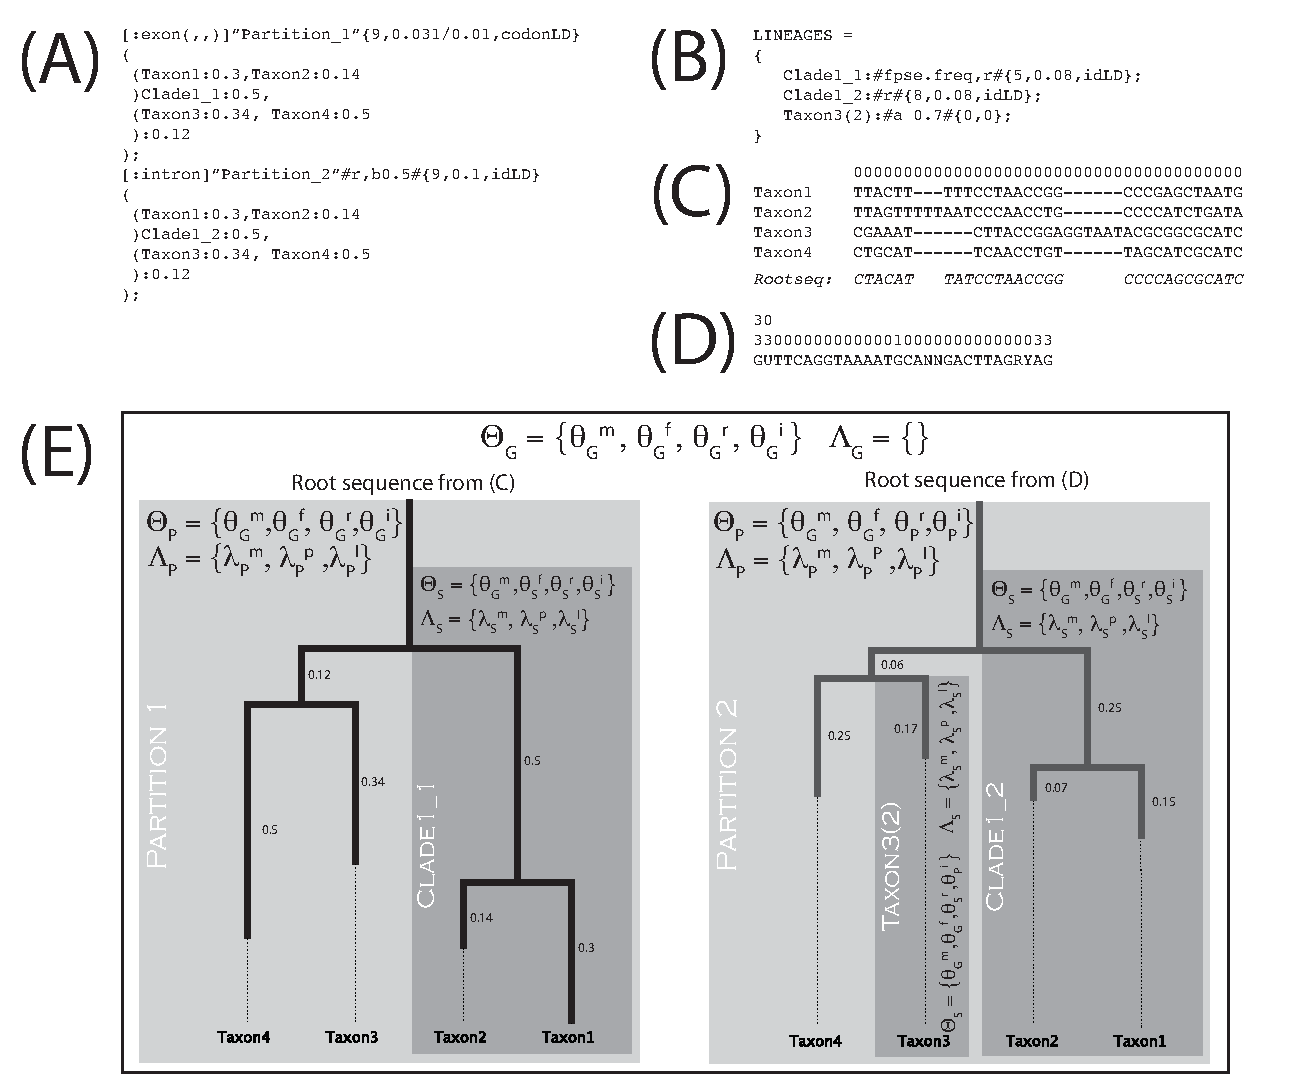
\includegraphics[width=\textwidth]{fig/general_simulation}
\caption{\textit{Depiction of simulation parameters and environments using the exon\_intron\_lineage example above, ``\texttt{./indel-seq-gen -m HKY -c 2,1,8 --lineage exon\_intron\_lineage.spec < exon\_intron\_lineage.tree}''. (A) The \texttt{exon\_intron\_lineage.tree} file specifies two partitions, ``Partition 1'' and ``Partition 2''. (B) The \texttt{exon\_intron\_lineage.spec} file specifies environment changes for the subtrees in (E). (C) The file \texttt{exon}, a multiple alignment input for partition~1. The final root sequence is shown below the alignment in italics. (D) The file \texttt{intron}, a root sequence input for partition~2. (E) The simulation run, showing the substitution ($\Theta_X$) and indel ($\Lambda_X$) settings, where $X$ specifies which environment the settings come from: $G\rightarrow$ global, $P\rightarrow$ partition, and $S\rightarrow$ subtree.}}
\label{fig:simulation_run}
\end{figure}


\subsection{Global Options}
\label{sec:global_options}
 To run indel-Seq-Gen from the command prompt, type the following line:
  
  \begin{verbatim}
  indel-seq-gen -m <matrix> [-options] < guide_tree_file > outfile
  \end{verbatim}

 \noindent Notes:
 \begin{itemize}
 \item This assumes that {\tt indel-seq-gen} is in your {\tt PATH} and data files locations are specified relative to your present working directory,
 \item The {\tt guide\_tree\_file} is described in Section~\ref{sec:partition_options}
 \item The ``{\tt $>$ outfile}'' portion of the command  specifies that all non-error messages generated by {\tt indel-Seq-Gen} will be saved in {\tt outfile}. Otherwise, messages will be displayed on the screen. 
\begin{GUI}
\item When using the GUI, this output will be saved in the outfile {\tt sim\_log\_file.txt}. This file is not overwritten; output for subsequent simulation runs are appended to this file.
\end{GUI}

 \end{itemize}

 \noindent {\tt indel-Seq-Gen} has many options. We suggest that you run some of the examples shown in Section~\ref{sec:example}. All necessary files are included in the provided {\tt \iSGcurrent/data} directory.  If you get any error message and the program does not run, please make sure if you followed the steps explained in the previous section. If you still cannot run the program, please contact us. The contact information is found in the first page.

\begin{ThreePartTable}
\begin{TableNotes}
\item[a] EV refers to the environment variable of which the global option is categorized. If left unspecified, the option does not refer to any of the environment variables. Environment variables are explained in Section~\ref{sec:overview}.
\item[b] Relative rates apply to the GTR matrix, not site rates.
\end{TableNotes}
 \begin{longtable}{p{0.40in}llp{2.75in}p{0.25in}}
 \caption{\textit{Global options (entered at the command line) and their effects for the indel-Seq-Gen run.  Subsequence options (described in the next Section) will override the global options if there are conflicts. For input type \{{\it list}\}, {\bf do not} use spaces to separate list items.}}\\
 \hline
 Option & Long Option & Type & Effect & EV\tnote{a}\\
 \hline
 \endfirsthead
 \caption[]{(continued)}\\
 \hline 
 Option & Long Option & Type & Effect & EV\tnote{a}\\
 \hline
 \\
 \endhead
 \hline
 \\
 \multicolumn{4}{l}{{\it Continued on next page...}}
 \endfoot
 \insertTableNotes
 \endlastfoot
\\
 -a & {\tt --}alpha & \{\it float\} & Shape (alpha) for gamma rate heterogeneity. Used only for DNA sequences. & $\theta^r$\\
\\
 -b & {\tt --}branch\_scale & \{\it float\} & Scaling factor for all branch lengths in simulation guide tree [default = 1.0].\\
\\
 -c & {\tt --}codon\_rates & \{\it list\} & \#1, \#2, \#3 = rates for codon position heterogeneity. Example: -c 0.15,0.05,0.8. Numbers are not required to sum to 1, as \iSGcurrentshort will normalize them. Used only for DNA sequences. & $\theta^r$\\
\\
 -d & {\tt --}select\_outputs & {\it \{0|1\}[6]} & Six binary numbers used to select which files to output. The file selection order is \{root, seq, ma, tree, trace, verb\}, i.e., to select only the ``.ma'' file, use option -d 001000 on the command line. {\it Must be used in conjunction with -e option.}
\\
 -e & {\tt --}outfile & \{\it string\} & Base filename for output files: $<$filename$>$.root, $<$filename$>$.seq, $<$filename$>$.ma, and $<$filename$>$.trace. These files will be created to hold the root sequences, sequence files, multiple alignments, and traced events output from the run, respectively.\\
\\
 -f & {\tt --}frequencies & \{\it list\} & Frequencies for individual amino acids (20, ARNDCQEGHILKMFPSTWYV) or nucleotides (4, ACGT), separated by commas, with \textbf{no spaces} between. Use ``e'' to for equal frequencies (0.05 or 0.25 for each state, respectively) [default = use frequencies based on the substitution matrix]. Example: -f 0.2,0.2,0.3,0.3 for 20\% A and 20\% C. & $\theta^f$\\
\\
 -g & {\tt --}num\_gamma\_cats & \{\it int\} & Number of categories for the discrete gamma-distribution rate heterogeneity. Must be between 2 and 32 [default = none]. Higher numbers of discrete categories severely affect the speed of iSGv2. & $\theta^r$\\
\\
 -h & {\tt --}help & & Output the usage instructions\\
\\
 -i & {\tt --}invar & \{\it float\} & Proportion of invariable sites [default = none]. & $\theta^i$\\
\\
 -k & {\tt --}lineage & \{\it filename \} & Subtree specification file name. See Section~\ref{sec:lineage}.\\
\\
 -j & {\tt --}step\_type & \{\it des, trs, gil\} & des = discrete evolutionary steps [default], trs = time relative steps, gil = Gillespie algorithm used for indel creation (fast). These are described below, in Section~\ref{sec:trace}.\\
\\
 -m & {\tt --}matrix & \{\it string\} & Substitution matrix: HKY, F84, GTR for nucleotides, PAM, JTT, MTREV, CPREV for amino acids. If using GTR, the relative rates must also be specified (option -r). & $\theta^m$\\
\\
 -n & {\tt --}num\_runs & \{\it int\} & The number of datasets to simulate for each tree [default = 1].\\
\\
 -o & {\tt --}outfile\_format & \{\it char\} & Output format: either Phylip (p), NEXUS (n), or FASTA (f) [default = Phylip]. \\
\\
 -q & {\tt --}quiet & & Quiet mode: only the root sequence, resultant sequences, and multiple alignment are printed.\\
\\
 -r & {\tt --}rel\_rates & \{\it list\} & Six comma-separated numbers specifying GTR rate matrix, in the following order: A to C, A to G, A to T, C to G, C to T and G to T. DNA only. & $\theta^m$ \tnote{b}\\
\\
 -s & {\tt --}option\_width & \{\it int\} & The number of residues per line on the multiple alignment output [default = 60]. \\
\\
 -t & {\tt --}tstv & \{\it float\} & Transition-transversion ratio. \\
\\
 -T & {\tt --}perturb\_tree & \{\it float\} & Rescales each branch length by a random factor $\in$ [1/{\it float}:{\it float}]. Perturbation of branches is different for each simulation run for multi-set simulations. \\
\\
 -u & {\tt --}indel\_fill & \{\it string\} & Insertion fill model, based on neighbor effects (preferring certain amino acids based on the neighboring amino acids): xia = original from~\cite{Xia02}, built on the E. coli K-12 proteins, sp = swiss-prot, ran = no neighbor effect [default = ran]. \\
\\
 -w & {\tt --}write\_anc & & Write ancestral sequences. \\
\\
 -z & {\tt --}rng\_seed & \{\it int\} & Manually set the random number seed.\\
\\
 -1 & {\tt --}proportion\_motif & \{\it float\} & The proportion of a random root sequence to be set as PROSITE regular expression motifs (as of PROSITE v20.60, 1038 patterns).\\
 \\
 \hline
 \label{tab:global}
 \end{longtable}
\end{ThreePartTable}

\newpage

 \subsubsection{Discrete steps and Trace file}
 \label{sec:trace}
 
 \iSGcurrentshort has two discrete-stepping methods and one non-discrete stepping method. Discrete stepping methods are implemented because (i) There is currently no continuous model for indel evolution, and thus most current simulation methods simulate with a flawed indel representation, and (ii) discrete steps allow for concrete tracking of events during the simulation (refer to~\cite{Strope09}). However, such methods are slow, and impractical for very large simulation runs. Thus, \iSGcurrentshort also includes a new non-discrete stepping method that also fixes the flaw in indel representations. These methods are described below.
 
 \paragraph{Discrete Stepping Methods:} 
 \begin{itemize} 
 \item The Discrete Evolutionary Steps (DES) model simply calculates $\epsilon$, and simulates sequences along the guide tree in $\epsilon$ step sizes. 
 \item Event occurrence times can be related along the simulation guide tree with the \emph{time relative steps}, or TRS, representation. \iSGcurrentshort scales the branch lengths of the guide trees and branch-specific $\epsilon$'s so that all mutation events that occur in simulation run are ordered with respect to the relative time of the run (i.e., the simulation starts at relative time point 0.0, and all taxa end at time point 1.0). 
 \end{itemize}
 
 \paragraph{Non-Discrete Steps:} The DES and TRS methods of simulation are computationally intensive, and can take a very long time for large datasets. For this reason, {\tt indel-Seq-Gen} also allows the user to choose an indel creation procedure that utilizes the Gillespie algorithm (GIL), as described by Cartwright~\cite{Cartwright05}. Using the GIL of indel creation greatly speeds up the the simulation time, and the output of such runs is comparable to the TRS method (i.e., the indel events are still traced). {\bf WARNING: If you choose to change the amino acid/nucleotide frequencies along lineages, DO NOT use this option. Use either DES or TRS.} The DES and TRS options will immediately begin shifting the amino acid/nucleotide distributions, while the GIL option will shift the distributions gradually.
 
 \subsubsection*{Event Tracking}

 A benefit introduced by the above methods is the ability to track indel events by the following properties:
 \begin{enumerate}
 \item ID
 \item Relative time of occurrence (from 0.0 (root of guide tree) to 1.0 (tips of guide tree); for the TRS model), 
 \item Set of taxa affected by change (i.e., subtree of occurrence), 
 \item Event type (insertion/deletion), 
 \item Indel length, and 
 \item Locations (columns) in the output MSA that reflect the event. 
 \end{enumerate}
 
 The time of occurrence for events is listed in different ways for each model: DES reports events by sequence partition (specified in the {\tt guide\_tree\_file} in the order they occur. TRS and GIL reports events by the relative time they occur in the guide tree. 
 
 
 %%%%%%%%%%% This is probably superfluous. %%%%%%%%%%%%%%%%
 %For example, see Figure~\ref{fig:input_MA}. Assuming a phylogeny that groups (Taxon1,Taxon2) and (Taxon3,Taxon4), positions 16--18 could have occurred in two ways, shown in Figure~\ref{fig:des}.
 %\begin{figure}
 %\verb+bit(0) = Taxon1+\\
 %\verb+bit(1) = Taxon2+\\
 %\verb+bit(3) = Taxon3+\\
 %\verb+bit(4) = Taxon4+\\~\\
 %\begin{tabular}{llllll}
 %{\tt [X,I,,1100,3,16:17:18]} & OR &
 %{\tt [X,D,,0011,3,16:17:18]} & OR &
 %{\parbox{1.5in}{\tt [X,D,,0011,1,17]\\
 %{\tt [Y,I,,1100,2,16:18]}}}\\
 %\end{tabular}
 %\caption{\textit{Three different ways that the events in Figure~\ref{fig:input_MA} could have occurred, as shown by the trace file using the discrete evolutionary steps (DES) paradigm, where {\tt X} is the unique event number describing the change. Since this is using DES, note that the relative time field is left empty.}}
 %\label{fig:des}
 %\end{figure}

\subsection{Partition Options}
\label{sec:partition_options}

 Specifications for each partition are given in the {\tt guide\_tree\_file}. Specifications for each partition are separated by `;'. Refer to the Examples section (Section~\ref{sec:example}) for some sample tree files.\\

 Partition options allow the user to create subsequence-specific effects by overriding the global parameters for specific subsequences. Partition options are shown in Table~\ref{tab:options}.

\begin{figure}
 \begin{small}
 \begin{tabular}{c|lcrlcrlcrlcrlcr}
 \hline
 \hline
  & \multicolumn{15}{c}{\underline{Partition-specific Parameters}}
  \\

  & \multicolumn{3}{c}{\textsc{Root Sequence}}
  & \multicolumn{3}{c}{Name}
  & \multicolumn{3}{c}{Substitution} 
  & \multicolumn{3}{c}{Indel}
  & \multicolumn{3}{c}{\textsc{Guide Tree}}
  \\
 \hline
\\
 \textit{Partition 1} & 
 \textbf{[}  & \textsc{Root Sequence 1} & \textbf{]} &
 \textbf{``} & Label 1         			& \textbf{''} &
 \textbf{\#} & Substitution 1  			& \textbf{\#}&
 \textbf{\{} & Indel 1         			& \textbf{\}} &
 \textbf{(}  & \textsc{Tree 1}          & \textbf{)};
 \\
 \\
 \vdots &
 \textbf{[}  & \vdots & \textbf{]} &
 \textbf{``} & \vdots & \textbf{''} &
 \textbf{\#} & \vdots & \textbf{\#}&
 \textbf{\{} & \vdots & \textbf{\}} &
 \textbf{(}  & \vdots & \textbf{)};
 \\
 \\
 \textit{Partition $n$} &
 \textbf{[}  & \textsc{Root Sequence $n$} & \textbf{]} &
 \textbf{``} & Label $n$         		  & \textbf{''} &
 \textbf{\#} & Substitution $n$  		  & \textbf{\#}&
 \textbf{\{} & Indel $n$                  & \textbf{\}} &
 \textbf{(}  & \textsc{Tree $n$}          & \textbf{)};
 \\
 \\
 \hline
 \hline
 \end{tabular}
\end{small}
\caption{\textit{A template of the guide tree file for a sequence with $\mathrm{n}$ partitions/subsequences. Parameters in small-caps are required, others are optional. Parameter values are listed in Table~\ref{tab:options}.}}
\end{figure}

\begin{small}
\begin{ThreePartTable}
\begin{TableNotes}
\item[a] EV refers to the environment variable of which the global option is categorized. If left unspecified, the option does not refer to any of the environment variables. Environment variables are explained in Section~\ref{sec:overview}.
\item[b] This option is used to specify an intron from an exon. This assumes that the global option `\texttt{-c}' (i.e., `\texttt{--codon\_rates}') is set. This flag sets the codon rates back to uniform rates.
\end{TableNotes}
\begin{longtable}{p{2cm}p{5.5cm}p{0.8cm}p{7cm}}
\caption{\textit{\normalsize Partition options.}}
\endfirsthead
\caption[]{{\normalsize (continued)}}\\
\hline 
\multicolumn{1}{|r}{{\normalsize Options}} & \multicolumn{1}{c}{{\normalsize Command Styles}} & EV\tnote{a} & \multicolumn{1}{c|}{\normalsize Description} \\
\hline
\\
\endhead
\hline\\
\multicolumn{2}{l}{\it \normalsize Continued on next page...}
\endfoot
\insertTableNotes
\endlastfoot
\hline

\multicolumn{1}{|r}{\normalsize Options} & \multicolumn{1}{c}{\normalsize Command Styles} & EV\tnote{a} & \multicolumn{1}{c|}{\normalsize Description} \\
\hline
\\
 \multicolumn{1}{r}{\it rootseq} 
 & \parbox[t]{5.4cm}{
  $\mathtt{[}$:$<$root\_sequence\_file$>\mathtt{]}$ or \\
  $\mathtt{[}$:$<$root\_sequence\_file$>$, \#$\mathtt{]}$ or \\
  $\mathtt{[}$:$<$mult\_align\_file$>(1,2,3)\mathtt{]}$ or \\
  $\mathtt{[}$:$<$mult\_align\_file$>(1,2,3)$, \#$\mathtt{]}$ or \\
  $\mathtt{[}$length$\mathtt{]}$ or \\
  $\mathtt{[}$length, \#$\mathtt{]}$
 } &
 & Six formats are allowed: The first two formats specify the root sequence file, in which a single root sequence along with the quaternary invariable array and any motifs/lineages are specified. The third and fourth format specify that the root sequence will be created from a file containing an input the multiple alignment file, with the quaternary invariable array and motifs/lineages specified. Sub-options `1', `2', and `3' specify the range of the multiple alignment to use, the number of sequences to select from the alignment, and the method of creating the consensus root sequence, respectively (for further details, see Section~\ref{sec:root}). The last two formats take as input a numeric value (not preceded by `:'), and generate a random sequence of the given length to use as the root sequence. When using the options with `\#', relative rates will be assigned to each partition. Using the `\#' option should be done only when the trees for each partition are the same.\\
\\

 \multicolumn{1}{r}{\it label}   
 & ``Partition Label'' && This option, when present, will label the boundaries of the subsequence in the multiple alignment in the {\tt *.verb} file with the name given. \\
\\

 \multicolumn{1}{r}{\it subseq}  & \parbox[t]{5.4cm}{
  \#i$<$\% invariable$>$,\\
  b$<$branch scale$>$,\\
  f$<$AA frequency file$>$,\\
  m$<$substitution matrix$>$,\\
  r\#
 } &
 \parbox[t]{0.7cm}{$\theta^i$\\
  \\
  $\theta^f$\\
  $\theta^m$\\
  $\theta^r$ \tnote{b}
 }
 & Option `b' modifies and options `i',`f',`m',`r' replaces the global options given at the command line, respectively. Option `b' will modify the default branch length scale by the value given. Option `r' is a flag that specifies that no site-specific rates are used for this partition (i.e., codon, gamma, and discrete gamma rates are reset to uniform rates). This is helpful for specifying introns in coding region sequences, as shown in~\ref{sec:coding_region}. Multiple options should be separated by commas.\\
\\
 \multicolumn{1}{r}{\it indel}   
 & \parbox[t]{5.4cm}{
  Format:\\
  \begin{tabular}{p{0.05cm}l}
  \multicolumn{2}{l}{\{\#$_1$, \#$_2$\textit{, $<$file$_1\!>$/$<$file$_2\!>$}\}} \\
  \multicolumn{2}{l}{\#$_1$: Max indel size}\\
  \multicolumn{2}{l}{\#$_2$: Indel probability distribution}\\
   & {\small If \#$_2$ = 0: Use Chang \& Benner}\\
   & {\small If \#$_2 > 0$: P(ins)=P(del)=\#$_2$} \\
   & {\small If \#$_2$/\#$_3$: P(ins)=\#$_2$, P(del)=\#$_3$}\\
  \multicolumn{2}{l}{\textit{$<$file$_1\!>$/$<$file$_2\!>$}} \\
\end{tabular} 
 } &
 \parbox[t]{0.7cm}{~\\
   ~\\
   $\lambda^m$\\
   $\lambda^p$\\
   ~\\
   ~\\
   ~\\
   $\lambda^l$
 }
 & \parbox[t]{7cm}{These options specify the different indel models and parameters.  Only the first two parameters are required. The last parameter, $<$file$_1$$>$/$<$file$_2>$, can be used to specify the two file names, which provide the user defined insertion length distribution (file$_1$) and deletion length distribution (file$_2$). If no distribution file is provided, the distributions given by Chang and Benner (2004) will be used. If only one distribution file is given, it will be used for both insertions and deletions.
 }\\ 
\\ 
 \multicolumn{1}{r}{\it Guide tree}          & Modified Newick Format && The rooted evolutionary tree for the partition. Trees must have the same number of taxa, with each taxon named the same in all trees for all partitions. The branching pattern as well as branch lengths, however, may vary. Branch lengths are assumed to be the expected number of substitutions per site. {\bf Taxon names cannot begin with a number}. Subtrees can be named inside of the tree, as shown in Figure~\ref{fig:newick_clades}.\\ \\
\hline 
\label{tab:options}
\end{longtable}
\end{ThreePartTable}
\end{small}

 \subsubsection{Specifying Subtrees in Newick Format}

 To specify subtrees for lineages and motifs, the Newick Tree Format must be clade-labelled, as shown in Figure~\ref{fig:newick_clades}. For multi-partition simulation runs, note that internal node clade labels can be named arbitrarily, thus for a particular subtree, each partition can have a unique lineage-specific parameterization (e.g., Clade1\_1 for partition 1, Clade1\_2, for partition 2, \ldots). However, since taxon labels \emph{must} be consistant between partitions, unique subtree parameters cannot be made (e.g., specifying {\tt Taxon1} is ambiguous if more than one partition is used). To specify partition-specific taxon subsequence parameters, refer to Figure~\ref{fig:newick_clades} for the method of specifying subtrees for taxon subtrees.
 
 \begin{figure}
  \begin{tabular}{p{2in}p{4in}}
  \begin{minipage}{2in}
   \verb+(+\\
   \verb+ (+\\
   \verb+  (Taxon1:0.1,Taxon2:0.1+\\
   \verb+  )Clade2:0.1,Taxon3:0.1+\\
   \verb+ )Clade1:0.1,+\\
   \verb+ (+\\
   \verb+  (Taxon4:0.1,Taxon5:0.1+\\
   \verb+  )Clade4:0.1,Taxon6:0.1+\\
   \verb+ )Clade3:0.1+\\
   \verb+);+\\
  \end{minipage}
  &
  \begin{minipage}{4in}
	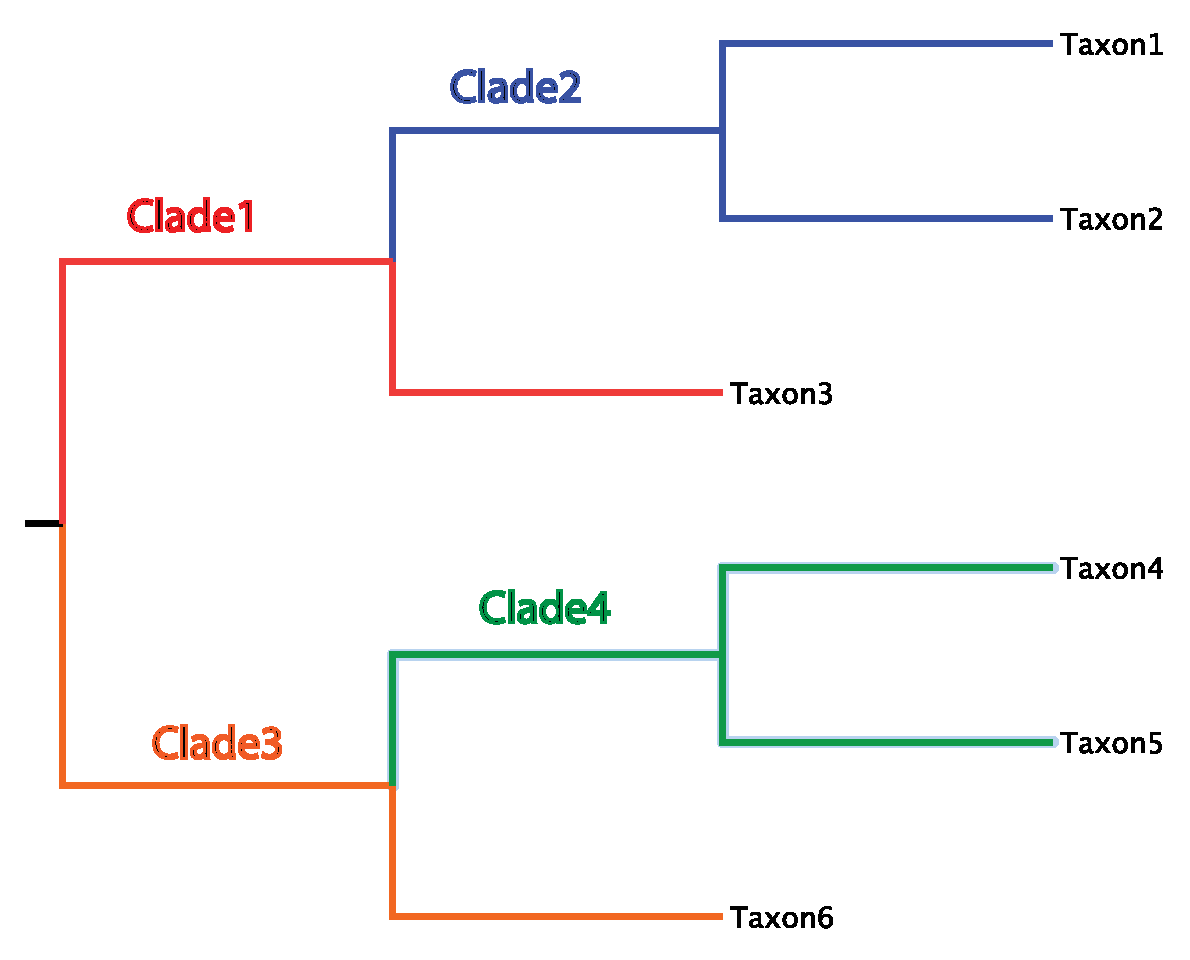
\includegraphics[width=4in]{fig/lineage_tree.eps}\\
  \end{minipage}
  \end{tabular}
 \caption{\textit{The subtree-labelled Newick format tree (left) and the resulting tree, which is colored to show the branches affected by the subtree label.}}
 \label{fig:newick_clades}
 \end{figure}

\begin{figure}[htbp]
 \centering 
 \begin{tabular}{lll@{ : }l}
 \hline
 Node Type & \multicolumn{3}{l}{Specification} \\
 \hline	
 Internal Node & $<$clade\_list$>$ && options; \\
 Taxon & $<$Taxon\_name$>$ && options; \\
 Taxon & $<$Taxon\_name$>$ & (partition\_list) & options;\\
 \hline
 \end{tabular}
 \caption{\textit{The format of subtree specification in \iSGcurrentshort.}}
 \label{fig:lineage_input}
 \end{figure}

 \subsection{Lineage and Motif Options}
 \label{sec:lineage}
 \label{sec:lineage_options}
 \label{sec:motif_options}
 Lineages and motifs are input to \iSGcurrentshort through the use of the global option ``{\tt -k}'' or ``{\tt --lineage}'' accompanied by the name of the lineage/motif file. This file consists of two parts: 
  \begin{enumerate} 
   \item LINEAGES, which change the conditions under which a subtree evolves, and 
   \item MOTIFS, which impose site-specific functional constraints on specific sequence positions for a specific subtree. 
  \end{enumerate}
 
The basic outline of this file is:
\begin{verbatim}
LINEAGES =
{
    subtree_list: "lineage_name"#subseq#{indel};
    .
    .
    .
}

MOTIFS =
{
    subtree:
        MARKER=<marker>;
        NAME=<motif_description>;
        PATTERN=<modified_PROSITE_motif>;
    .
    .
    .
}
\end{verbatim}

Lineages and motifs both work on subtrees (internal nodes named in input guide tree). To make a lineage or motif effective from the root of the guide tree, name {\tt subtree\_list} in LINEAGES or {\tt subtree} in MOTIFS as {\tt subtree:} to {\tt root:}, respectively. 


 \subsubsection{LINEAGES}
 Lineages allow for a specific subtree to evolve under different conditions as specified for partitions in the tree file.  Subsequence options (\#\#) are the only set of options affected by these restrictions, shown in Table~\ref{tab:lineage_options}. Labelling (``'') and indel (\{\}) options are no different than in partitions. {\it Note: In order to remove indels from a lineage, include the option \{0,0\} in the lineage.} 
 \iSGcurrentshort prohibits unrealistic changes, {\it e.g.} when changing site rates (gamma rates ($\gamma$), discrete gamma rates, codon rates, and uniform rates), \iSGcurrentshort only allows a subset of ancestor$\rightarrow$descendant category changes: $\gamma\rightarrow$\{$\gamma$, uniform\}, discrete $\gamma\rightarrow$\{discrete $\gamma$, uniform\}, codon$\rightarrow$\{codon, uniform\}, and uniform$\rightarrow$\{$\gamma$, discrete $\gamma$, uniform\}.
 
 \begin{threeparttable}
  \caption{\textit{Novel functions and restrictions imposed for lineage-specific subsequence options (\#\#).}}
  \begin{tabular}{p{0.1in}lp{2.25in}p{2.25in}p{0.5in}}
  \hline\hline
  & Option: & Restrictions & Function & EV\tnote{a}\\
  \hline
   \multicolumn{4}{l}{\it Site rates:} \\
   & a & Partition must be either gamma, discrete gamma, or uniform rates. & Change $\alpha$ parameter for gamma site rates. & $\theta^r$\\
   & c & Partition must be codon rates. & Change codon position frequencies. & $\theta^r$\\
   & g & Partition must be discrete gamma or uniform rates. & Change the number of discrete categories. & $\theta^r$\\
   \multicolumn{4}{l}{\it Other:} \\
   & b & Cannot change branch scale. & None. \\
   & f & None. & Change character frequencies. & $\theta^f$\\
   & i & Only affects random input sequence (i.e., [100]) & Change percentage invariable. & $\theta^i$\\
   & m & Must be a matrix used for specifiec character set (nucleotides vs. amino acid), cannot take value GTR. & Change substitution matrix. & $\theta^m$\\
   & r & None. & Removes \emph{all} constraints (e.g., invariable sites, motifs, site rates) from a lineage, effectively making all changes in the lineage occur using uniform rates. & $\theta^r, \theta^i$\\
  \hline\hline
  \end{tabular}
  \begin{tablenotes}
  \item[a] EV refers to the environment variable of which the global option is categorized. If left unspecified, the option does not refer to any of the environment variables. Environment variables are explained in Section~\ref{sec:overview}.
  \end{tablenotes}
  \label{tab:lineage_options}
 \end{threeparttable}
 
 \subsubsection{MOTIFS}

 Two steps are required to specify a motif: (1) Marking the root sequence in the \textit{rootseq} file (as in Table~\ref{tab:options}, formats 1--4), and (2) Specifying constraints in the lineage file. 

  \paragraph{Motif types:} \iSGcurrentshort allows two formats for motifs: PROSITE-like motif format and sequence template motif format. PROSITE-like motif format specifies any length of motif that follows the PROSITE regular expression pattern. Sequence template motif format is required to cover the entire sequence, and are used to place minimum and maximum length parameters on subsequences.
 
  \paragraph{Specifying sites on root sequence:} Marking sites is done in the root sequence input file, below the input root sequence or input multiple alignment. To begin marking the sequence, place a `*' corresponding to the first position in the root sequence. This \emph{must} be present for motifs to be correctly parsed. All other positions in the input root sequence must have a corresponding `*' or motif label (anything but `*'). Motif specification characters also must be contiguous, i.e., after specifying the positions that are in a motif, the rest of the motif specification line must be `*'s. As a regular expression, the PROSITE-like motif specification is: *$^+x^+$*$^*$, where $x$ is the character for the motif specification. For template-like motifs, the regular expression is *$[0-9]^n$\footnote{For multiple sequence alignment input, the regular expression is *$[[0-9],.]^n$, see Section~\ref{sec:ma_root} for details.}, where $n$ is the length of the root sequence input. There is no limit to the number of motifs that can be specified on a root sequence. Figure~\ref{fig:motif_errors} shows some errors that can be made in specifying motifs.
  
 \begin{figure}[htbp]
  \begin{tabular}{lp{2.5in}p{2.5in}}
   \hline\hline
   Motif specification & Error & Fix\\
   \hline
   {\tt aaaaa***************} & Motif specification must begin with `*'\\\\
   {\tt *aaaaaa******aaaaa**} & Motif specification must be contiguous & split motif into 2 motifs, specifying each area, or make entire motif contiguous.\\\\
   {\tt *******aaaaaabbbbb**} & Can only use one motif marker per motif specification & split motif into 2 motifs, specifying each area, or make entire motif contiguous.\\\\
   \hline
  \end{tabular}
  \caption{\textit{Erroneous motif specifications for a root sequence of length 20, with the assumption that the motif is labelled by `a'.}}
  \label{fig:motif_errors}
 \end{figure}
 
  \paragraph{Specifying motif constraints:} After the motif-participating sites are labelled in the root sequence, specify the conditions that apply to each site in the lineage file. The fields for specifying motifs are shown in Table~\ref{tab:motif_spec}. 

  \begin{table}
   \caption{\textit{List of the options for specifying motifs. See Figure~\ref{fig:lipocalin_motif} for an example of a motif specification.}}
   \begin{tabular}{p{0.1in}p{1in}p{3in}p{1.5in}}
	\hline\hline
	\multicolumn{2}{l}{Field} & Description & Motif type \\
	\hline
    \multicolumn{2}{l}{MARKER} &  A single character, value can be anything except for the character `*' (see Section~\ref{sec:root} for specifying sites for motif).  This is the ID of the motif as specified in the root sequence input. & Prosite-like, template (0-9 only). \\\\
    \multicolumn{2}{l}{NAME} & Not required. This is the description of the motif. & Prosite-like, template\\\\
    \multicolumn{2}{l}{PATTERN} & Regular expression patterns, as below.\\
	 & {\tt [list]} & A list of acceptable amino acids or nucleotides for a site, site can take value of {\tt list}. & Prosite-like \\\\
	 & {\tt \{list\}} & A list of unacceptable amino acids or nucleotides for a site, site can take any value \emph{not} in {\tt list}. & Prosite-like \\\\
	 & {\tt char} & Invariable site, takes value of {\tt char}. & Prosite-like \\\\
	 & x & Site can take any amino acid or nucleotide value. & Prosite-like, template \\\\
	 & x($n$) & Next $n$ sites can take any amino acid or nucleotide value. & Prosite-like, template \\\\
	 & x($min,max$) & Variable length motif sequence. Cannot start a motif with a variable length motif position. This specifies that length of the motif positions can vary between $m$ to $n$ sites (variance caused by indels). Variable sites cannot overlap between different motifs. & Prosite-like, template \\
	\hline
   \end{tabular}
   \label{tab:motif_spec}
  \end{table}

 Note that when marking motifs, the marked positions must be the same size as the PATTERN specified. In the case of variable positions, \iSGcurrentshort requires that the maximum size of the motif (i.e., $n$ in {\tt x$(m,n)$}) are represented in the root sequence. To make this possible, you may need to place `-' in the root sequence or root MSA, as shown in Figure~\ref{fig:lipocalin_motif}. If a character is placed in the variable motif instead of `-', \iSGcurrentshort will assume that this position is part of the variable motif in the root sequence.
 
 \begin{figure}
 \begin{tabular}{|l|}
 \multicolumn{1}{l}{\fbox{In root sequence specification file}}\\
 \multicolumn{1}{l}{\texttt{50}}\\
 \multicolumn{1}{l}{\texttt{00000000000000000000000000000000000000000000000000}}\\
 \multicolumn{1}{l}{\texttt{ASPISTIQAATVPDSS--EVAGKWYIVALASNTSFLREKGKMKMVMARIL}}\\
 \multicolumn{1}{l}{\texttt{*************bbbbbbbbbbbbbb***********************}}\\
 \multicolumn{1}{l}{}\\
 \hline
 \fbox{In motif specification file}\\\\
  $<$subtree$_i>$:\\
   \verb+    MARKER=b;+\\
   \verb+    NAME=PS00213: Lipocalin signature, ALL;+\\
   \verb+    PATTERN=[DENG]-{A}-[DENQGSTARK]-x(0,2)-[DENQARK]-[LIVFY]-{CP}-G-{C}-W-[FYWLRH]-{A}-[LIVMTA];+\\
 \hline
 \end{tabular}
 \caption{\textit{An example of the specifying the lipocalin motif in the single root sequence input. The pattern in the motif specification file corresponds to the marked sites in the last line of the root sequence file. The sites corresponding to {\tt x(0,2)} in this instance is specified as 0 sites, with the `-' placeholder being used to fill the maximum possible number of sites (2) that could occupy the ``variable-length site''.}}
 \label{fig:lipocalin_motif}
 \end{figure}

\section{Root Sequence Input}
\label{sec:root}

The root sequence is specified by the square brackets ({\tt [ ]}) in the guide tree file. There are three parameters, if used, for root sequence input:
\begin{enumerate}
\item Specifying the length of root sequence. indel-Seq-Gen will randomly generate a root 
sequence of the specified length.  For example {\tt [40]} calls for a root sequence of length 40 characterss.
\item Root sequence input.
\item Multiple alignment input.
\end{enumerate}

Each of these options is explained in the following subsection. Make sure that the input file is in the same directory when using a root sequence input file (options 2 and 3).

\subsection{Root Sequence Input}

This option specifies that the user has a root sequence in a file for a partition.  

In the tree file, the root sequence input is specified as:
\begin{verbatim}
[:<rootseq_file>]
\end{verbatim}

The format of the file \verb+<rootseq_file>+ is:
\begin{verbatim}
<length of sequence>
<invariable array>
<sequence>
<motif_spec>
\end{verbatim}

Figure~\ref{fig:trx} gives an example of a root sequence for conserving a Thioredoxin-fold 
protein sequence motif.

\begin{figure}[btph]
 \centering
  \begin{tabular}{|l|p{1in}|l|}
  \cline{1-1}\cline{3-3}
  \texttt{20} && \texttt{20} \\
  \texttt{00003223100000000000 } && \texttt{00000000100000000000 } \\
  \texttt{LARDCVLCSTWVTIALACLK } && \texttt{LARDCVLCSTWVTIALACLK } \\
   && \texttt{****aaaa************ } \\
  \cline{1-1}\cline{3-3}
  \multicolumn{1}{l}{}\\
  \multicolumn{1}{l}{}\\
  \cline{3-3}
  \multicolumn{2}{l|}{}&\fbox{In motif specification file}\\
  \multicolumn{2}{l|}{}&root:\\
  \multicolumn{2}{l|}{}&\verb+    MARKER=a;+\\
  \multicolumn{2}{l|}{}&\verb+    NAME=Trx-like;+\\
  \multicolumn{2}{l|}{}&\verb+    PATTERN=C-[GATPLVE]-[PHYWSTA]-C;+\\
  \cline{3-3}
  \end{tabular}
 \caption{\textit{Thioredoxin-fold (Trx-fold) proteins have a characteristic ``CXXC'' motif that is conserved for all proteins in the family. (Left): This root sequence input requires the CXXC motif to remain constant for all sequences created through the use of the invariable array (described later), listed above the root sequence. The serine in position 9 will also be held invariable, though insertions are allowed to occur between itself and the previous cysteine.  Finally, the length of the root sequence is given by the first line. Note that this sequence is not truly a Trx-fold sequence, but an example to show the usage of the invariable array. (Right): Motif specification of the Thioredoxin active site. Motif specifications preserve both the length dependence and character subsets. Note also that the invariable array is no longer used to preserve the motif; it is recommended that when using motif specification, all non-motif positions in invariable array should be set to 0.}}
\label{fig:trx}
\end{figure}

\subsection{Multiple Alignment Input}
\label{sec:ma_root}
This option specifies that the user has a multiple alignment of their sequence set, and wants a root sequence created from the multiple alignment. In the guide tree file, the root sequence input is specified as:
\begin{verbatim}
[:<ma_file>(1,2,3)]
\end{verbatim}

Where options 1, 2, and 3 stand for:
\begin{enumerate}
\item The range of the multiple alignment to use, where the format is {\it beginning}{\tt 
:}{\it end}.  An input of {\tt 21:67} specifies the range from the 21st to the 67th spot 
(inclusive) of the input multiple alignment.  Default for this option is the entire range of the multiple alignment. 
\item The number of sequences to choose from the multiple alignment.  indel-Seq-Gen randomly with replacement selects the specified number of sequences from the multiple alignment. Default for this option is to use all sequences.
\item Method for collapsing the multiple alignment into a root sequence, either random 
{\tt `r'} or consensus {\tt `c'}.  Consensus is a majority-rule method, using a coin flip to break ties.  Random uses a weighted coin toss based on the character composition at the site to choose the representative character, except for invariable positions, which will be chosen by consensus. For an example of the weighted coin toss, look at the first column in Figure~\ref{fig:input_MA} in which all sequences emit an amino acid, column 6.  In this 
column, there are 2 T's, 1 V, and 1 C.  A weighted coin toss on this column will be a T 50\% of the time, a V 25\% of the time, and a C 25\% of the time. The default for this option is consensus.
\end{enumerate}

When specifying the multiple alignment in the tree file, a blank field specifies that the default entry for the field is desired.  For example, \verb+[:input_MA(,,r)]+ indicates that the entire range and all sequences from {\tt input\_MA} will be used, but that the character that will represent the column will be chosen by a weighted coin toss based on the characters that appear in that column.  Note that the size of the root sequence can fluctuate between simulation runs.  For example, using the option \verb+[:input_MA(,1,)]+ will randomly choose a single sequence to create root sequence, thus the sequence that 
indel-Seq-Gen chooses will be the length of the root sequence for that subsequence.\\

Format:
\begin{verbatim}
<invariable array>
<sequence 1>
<sequence 2>
 .      .
 .      . 
 .      .
<sequence n>
<motifs>
\end{verbatim}

Figure~\ref{fig:input_MA} is an example of an input multiple alignment of the SET-C region of the SET-domain family. The `-' is the only character that will be accepted for the gap character. Irregular characters (``YRUN'' in nucleotides, ``BZJX'' in amino acids) cause each character for which they stand for to be counted as the 1 over the number of characters they represent (e.g., `B' increments both `N' and `D' by 0.5). All `.'s in the template \emph{must} also be `.'s in all motifs coinciding with the same site. The reverse, however, is fine, as shown in this example, in the position just before the GxxL motif.

\begin{figure}[Htbp]
\centering
\begin{tabular}{|l|}
\hline
\fbox{Input MA, using invariable array}\\
\verb+       0000000000000000000000000000000100322300010000+\\
\verb+Taxon1 -----TKEDF-----TSDQTNPIGQDSATRLILKGEELTCNYKLFD+\\
\verb+Taxon2 RNSCNVVPKIVQVNGDFRIRFTALRD-----IK-GEELFFNYGENF+\\
\verb+Taxon3 -----TGVSNNQFGG---YDFVALGD-----IE-GEELTWBYETTE+\\
\verb+Taxon4 -----CELVQLTEFS---LGVVAICN-----IE-GEELSFDYAWEA+\\
\hline
\multicolumn{1}{l}{}\\
\hline
\fbox{Input MA, using motif specification}\\
\verb+       0000000000000000000000000000000000000000010000+\\
\verb+Taxon1 -----TKEDF-----TSDQTNPIGQDSATRLILKGEELTCNYKLFD+\\
\verb+Taxon2 RNSCNVVPKIVQVNGDFRIRFTALRD-----IK-GEELFFNYGENF+\\
\verb+Taxon3 -----TGVSNNQFGG---YDFVALGD-----IE-GEELTWBYETTE+\\
\verb+Taxon4 -----CELVQLTEFS---LGVVAICN-----IE-GEELSFDYAWEA+\\
\verb+       *******************************bb.bbbb********+\\
\verb+       *....000000000000000000000..000000000000000000+\\
\hline
\multicolumn{1}{l}{}\\
\hline 
\fbox{In motif specification}\\
$<$subtree$>$:\\
\verb+    MARKER=b;+\\
\verb+    PATTERN=I-x-G-x(2)-L;+\\
$<$subtree$'>$:\\
\verb+    MARKER=0;+\\
\verb+    NAME=Multiple alignment template example;+\\
\verb+    PATTERN=x(10,22)-x(2,6)-x(5)-x(3,8);+\\
\hline
\end{tabular}
\caption{\textit{{\bf input\_MA}: (Top) An example of a 4 sequence multiple alignment from the SET-domain family of sequences using the invariable array.  The GXXL motif is conserved in both the invariable array, along with the tyrosine and isoleucine. (middle, bottom) The motif specification input and root sequence file. The motif will be conserved in the same manner as the invariable array on the top. However, specifying this subsequence as a motif allows the user to conserve the motif on a subtree, rather than over the entire guide tree as is done with the invariable array.}}
\label{fig:input_MA}
\end{figure}

 \subsubsection{Multiple alignment root sequence input for template motifs}
 
 Note that the multiple alignment root sequence input will have variable length, depending on the number of columns in the multiple alignment that are inferred to be gap columns ($>50\%$ `-' in a column). When specifying template motifs, all sites, except the first, must belong to a position in the template. For this reason, when specifying a template motif, \iSGcurrentshort also allows the character `.' on a position in the motif specification. The `.' character specifies that this site should be excluded from the template sites. For example, in Figure~\ref{fig:input_MA}, 6 positions of the multiple sequence alignment are excluded from the template specification.

\subsection{Invariable Array}

The invariable array in indel-Seq-Gen is a quaternary array that specifies how a region is 
allowed to evolve, and is specified in the root sequence input. Table~\ref{tab:invariable} 
shows the effect of each numerical entry in the invariable array, and Figure~\ref{fig:placement} shows an example of how the algorithm finds possible positions for indels based on the invariable array.

\begin{table}[Htbp]
\caption{\textit{Representation of positions in the invariable array, and effects on the sequence. Invariable sites (1 and 3) block both deletion and substitution of the corresponding position in the sequence array.  No-indel sites (2 and 3) block deletion of the sequence array, but also block insertion events from occurring between consecutive no-indel positions (between 2-2, 2-3, 3-2, and 3-3) in the invariable array.}}
\centering
\begin{tabular}{|l|c|}
\hline
\# & Effects \\
\hline
0 & None \\
1 & Invariable \\
2 & No-indel \\
3 & Invariable + No-indel  \\
\hline
\end{tabular}
\label{tab:invariable}
\end{table}

\begin{figure}[Htbp]
\begin{verbatim}
Accepting Positions:

  Invariable Array:       0 0 1 2 3 0
  Insertion (any size):  1 1 1 1 0 1 1

  Invariable Array:       0 0 1 2 3 0
  Deletion (size 1):      1 1 0 0 0 1
  Deletion (size 2):      1 0 0 0 0 0
  Deletion (size 3):      0 0 0 0 0 0

\end{verbatim}
\caption{\textit{The invariable array and accepting positions for insertion and deletion events. For insertions, the accepting positions (denoted by `1' and `0' above) are located in between consecutive positions in the invariable array, while deletion accepting positions correspond exactly those in the invariable array.  In the accepting positions, the site with `1' is allowed to have indels. In the rare case that an accepting position cannot be found (as in the size 3 deletion example above), indel-Seq-Gen will output an error, but continue the simulation run.}}
\label{fig:placement}
\end{figure}

\section{Other Input Files}

\subsection{Character Frequencies {\tt \#f{\it freq\_file}\#}}

Protein and nucleotide subsequences often evolve under different functional constraints, causing them to display different character frequencies. For this, a file containing 20 amino acid frequencies (order: ARNDCQEGHILKMFPSTWYV) or 4 nucleotide frequencies (order: ACGT) separated by commas can be entered for each subsequence with the option: 
\verb+#f<freq_file>#+.  Values from the input file are read and normalized to create a 
distribution, where the number of values is specified by the maximum indel size of the 
subsequence. For an example, see the file {\tt aaf.freq} included with all iSG {\tt .tar.gz} archive downloads.

\subsection{Indel Probabilities {\tt \{\#$_1$,\#$_2$,{\it indel\_file(s)}\}}}

Insertion and deletion frequencies can be provided for each subsequence.  The format of the file is shown in Figure~\ref{fig:zipf}.  This example is for the indel probabilities of sizes 1--10 of the Zipfian distribution described in Chang and Benner~\cite{Chang04}.  
indel-Seq-Gen will read in the number of values corresponding to the {\tt max\_indel\_size} (\#$_1$) specified for the subsequence (for Figure~\ref{fig:zipf}, the maximum indel size of a subsequence using this file can be up to size 10), and then normalize the values to create a distribution.  This means that the frequencies can be given in absolute numbers or in any scale (as shown in Figure~\ref{fig:zipf}).  If the maximum indel size is greater than the number of indel positions in the length distribution file, indel-Seq-Gen will output a message that it is unable to read the input distribution file.

\begin{figure}[htbp]
\centering
\fbox{\texttt{2628,743.8,355.5,210.5,140.2,100.6,76,59.6,48.1,39.7}}
\caption{\textit{An example length distribution input file.  This has the frequencies of indels with lengths from 1 to 10 amino acids, taken from the first 10 values of the Zipfian distribution.  The number of values in this file should not be smaller than the given max indel size.}}
\label{fig:zipf}
\end{figure}

\section{Examples}
\label{sec:example}

 \subsection{Basic coding and non-coding}
 Despite the complexity that exists in iSGv2, the main goal of the simulation method is to be an all-purpose sequence simulator. Therefore, included in the distribution is a file called ``{\tt simple\_nuc.tree}'', shown in Figure~\ref{fig:simple_nuc}. 
 
 \begin{figure}
 \fbox{\tt [999]((Taxon1:0.3,Taxon2:0.14):0.5,(Taxon3:0.34, Taxon4:0.5):0.12);}
 \caption{\textit{A simple example of a nucleotide simulation partition file. This simulates a 999 nucleotide sequence with no indels, along a guide tree of 4 taxa.}}
 \label{fig:simple_nuc}
 \end{figure}
 	
 Given this example, assume the usage of the Hasegawa, Kishino, and Yano~\cite{Hasegawa85} substitution matrix. The following two commands will create non-coding and coding simulation runs, respectively:
 \begin{verbatim}
 ./indel-seq-gen --matrix HKY --outfile DNA_out < simple_nuc.tree
 ./indel-seq-gen --matrix HKY --codon_rates 0.2,0.05,0.75 --outfile DNA_out < simple_nuc.tree
 \end{verbatim}

 This will also create five outfiles: DNA\_out.ma, DNA\_out.seq, DNA\_out.root, DNA\_out.trace, and DNA\_out.verb. In the first examples, the sites are mutated uniformly as is non-coding DNA. In the second example, the third coding mutates 75\% of the time, while the first and second codn mutate 20\% and 5\% of the time, respectively, mimicking codon position rates.

 \subsection{Including indels}

 A little more complex example including indels is shown in Figure~\ref{fig:mid_nuc}. Notice that we now need to two trees to represent coding or non-coding sequences, since indel sizes that are not a multiple of three would cause a nonsense mutation.
 
 \begin{figure}
 \begin{tabular}{|l|}
 \hline
 \fbox{mid\_nuc\_coding.tree}\\
 {\tt [999]\{9,0.1/0.3,codonLD\}((Taxon1:0.3,Taxon2:0.14):0.5,(Taxon3:0.34, Taxon4:0.5):0.12);}\\
 \hline 
 \multicolumn{1}{l}{}\\
 \hline
 \fbox{codonLD}\\
 {\tt 0,0,3222,0,0,233, 0,0, 0.23}\\
 \hline
 \multicolumn{1}{l}{}\\
 \multicolumn{1}{l}{}\\
 \hline
 \fbox{mid\_nuc\_noncoding.tree}\\
 {\tt [999]\{9,0.1/0.3,idLD\}((Taxon1:0.3,Taxon2:0.14):0.5,(Taxon3:0.34, Taxon4:0.5):0.12);}\\
 \hline
 \multicolumn{1}{l}{}\\
 \hline
 \fbox{idLD}\\
 {\tt 2628,743.8,355.5,210.5,140.2,100.6,76,59.6,48.1,39.7}\\
 \hline
 \end{tabular}
 \caption{\textit{The specification files for a simulation run with indels, and the associated files, codonLD and idLD.}}
 \label{fig:ORF}
 \end{figure}

 The commands:
 \begin{verbatim}
 ./indel-seq-gen -m HKY -e mid_noncoding --num_runs 5 < mid_nuc_noncoding.tree
 ./indel-seq-gen -m HKY -e mid_noncoding -n 5 -c 2,1,8 --invar 0.02 < mid_nuc_coding.tree
 \end{verbatim}

 In this example, the previously introduced options {\tt --matrix}, {\tt --outfile}, and {\tt --codon\_rates} have been replaced by their short options. The {\tt --num\_runs (-n)} option has also been included, so that five runs will be simulated. The multiple alignments of this example is very gappy, since in the indel options, the maximum indel size is 9 nucleotides, and an insertion occurs once for every 10 substitutions, a deletion once every 3.3 substitutions. Finally, the option {\tt --invar} sets 2 percent of the sites to be invariable. Codon rate input also does not need to add up to 1, as \iSGcurrentshort will normalize the values.
 
 \subsection{Coding and non-coding together}
 \label{sec:coding_region}

 \iSGcurrentshort has the unique ability to simulate exons and introns in a single run. This adds yet more complexity, as you can see by the necessary files, as listed in Figure~\ref{fig:ORF}. Files that remain the same as previous examples are excluded from this figure.
 
 \begin{figure}
 \begin{tabular}{|l|}
 \hline
 \fbox{exon\_intron.tree}\\
 {\tt [:exon(,,)]\{9,0.031/0.01,codonLD\}((Taxon1:0.3,Taxon2:0.14):0.5,(Taxon3:0.34, Taxon4:0.5):0.12);}\\
 {\tt [:intron]\#r,b1.2\#\{9,0.1,idLD\}((Taxon1:0.3,Taxon2:0.14):0.5,(Taxon3:0.34, Taxon4:0.5):0.12);}\\
 \hline
 \multicolumn{1}{l}{}\\
 \hline
 \fbox{exon}\\
 \verb+          000000000000000000000000000000000000000000+\\
 \verb+Taxon1    TTACTTT---TTCCTAACCGG---C---CCGAGCT---AATG+\\
 \verb+Taxon2    TTAGTTTTTAATCCCAACCTG---C---CCCATCT---GATA+\\
 \verb+Taxon3    CGAAATC------TTACCGGAGGTAATACGCGGCGC---ATC+\\
 \verb+Taxon4    CTGCATT------CAACCTGT---T---AGCATCGC---ATC+\\
 \hline
 \multicolumn{1}{l}{}\\
 \hline
 \fbox{intron}\\
 \verb+30+\\
 \verb+330000000000001000000000000033+\\
 \verb+GUTTCAGGTAAAATGCANNGACTTAGRYAG+\\
 \hline
 \end{tabular}
 \caption{\textit{The specification files for a simulation run of one exon partition and one intron partition with indels, and the associated root sequence files, exon and intron.}}
 \label{fig:mid_nuc}
 \end{figure}

 The command:
 \begin{verbatim}
 ./indel-seq-gen -m HKY -c 2,1,8 -e exon_intron --step_type trs < exon_intron.tree
 \end{verbatim}

 There are many interesting things to note:
  \begin{enumerate}
  \item Codon rates are input at the command line. The subsequence option \#r\# in the intron sequence resets the rates to uniform rates in the intron. The additional subsequence options \#b1.2\# multiplies all branch lengths in the tree by a factor of 1.2.
  \item The file {\tt intron} conserves the nuclear-like spliceosomal sites (GU at beginning, G in the middle, and AG at the end).
  \item The option {\tt --step\_type} sets the simulation run to be in time relative steps. The output file {\tt exon\_intron.trace} will contain where each indel event occurred and the relative time of the event, as explained in Section~\ref{sec:trace}.
  \end{enumerate}

 \subsection{Lineage Introduction}
 Lineages are one of the unique abilities of iSGv2, paricularly the ability to cause a lineage to evolve under no specifications, which we call ``pseudogene'' evolution (the {\tt p} option in subsequence options {\tt \#\#}). To add lineages to the previous example, we need to specify clades in the partition file, create the lineage file and specify this file on the command line. Figure~\ref{fig:lineage_spec} shows the file changes, and Figure~\ref{fig:lineage_output} shows the output of the command:
 
 \begin{verbatim}
./indel-seq-gen -m HKY --lineage exon_intron_lineage.spec --alpha 1.3 < exon_intron_lineage.tree
 \end{verbatim}

 No output files are given, thus the output is printed to the screen. Note that the file {\tt outfile.verb} will still be created. 

\begin{figure}
 \begin{tabular}{|l|}
 \hline
 \fbox{exon\_intron\_lineage.tree}\\
 \verb+[:exon(,,)]"Partition_1"{9,0.031/0.01,codonLD}+\\
 \verb+(+\\
 \verb+ (Taxon1:0.3,Taxon2:0.14+\\
 \verb+ )Clade1_1:0.5,+\\
 \verb+ (Taxon3:0.34, Taxon4:0.5+\\
 \verb+ ):0.12+\\
 \verb+);+\\
 \verb+[:intron]"Partition_2"#r,b0.5#{9,0.1,idLD}+\\
 \verb+(+\\
 \verb+ (Taxon1:0.3,Taxon2:0.14+\\
 \verb+ )Clade1_2:0.5,+\\
 \verb+ (Taxon3:0.34, Taxon4:0.5+\\
 \verb+ ):0.12+\\
 \verb+);+\\
 \hline
 \multicolumn{1}{l}{}\\
 \hline
 \fbox{exon\_intron\_lineage.spec}\\
 \verb+LINEAGES =+\\
 \verb+{+\\
 \verb+    Clade1_1:#fpse.freq,p#{5,0.08,idLD};+\\
 \verb+    Clade1_2:#r#{8,0.08,idLD};+\\
 \verb+    Taxon3(1):#a 0.7#{0,0};+\\
 \verb+}+\\
 \hline
 \multicolumn{1}{l}{}\\
 \hline
 \fbox{pse.freq}\\
 \verb+10,23,15,6+\\
 \hline
 \end{tabular}
 \caption{\textit{The specification of subtrees in exon\_intron\_lineage.tree and the corresponding specifications in exon\_intron\_lineage.spec. Subtrees on internal nodes can be uniquely named, thus the convention Clade\_$<$partition\_number$>$. Taxa cannot be uniquely specified between partitions, since they are required to be the same for all partitions. Thus, the taxon lineage (Taxon3) contains the list of partitions it is active in in parentheses. In this case, the lineage specifications for Taxon3 are active only for the first partition.}}
 \label{fig:lineage_spec}
\end{figure}

 Some finer points:
 \begin{enumerate}
 \item The global parameter {\tt --alpha} specifies that, unless otherwise specified in clades, all branches in all trees will evolve with site rates, where the gamma parameter $\alpha=1.3$. However, Clade1\_1 and Clade1\_2 both become pseudogene lineages, which releases site rates from them. Taxon3 in the first tree also does not evolve with this gamma, since the lineage file specifies it to evolve with $\alpha=0.7$ ({\tt \#a 0.7\#}).
 \item Taxon3, partition 1, evolves without indels (\{0,0\}).
 \end{enumerate}

\begin{figure}
\begin{verbatim}
>Dataset_0__partition_1
[0,D,,1100,4,16:17:18:19]
[1,I,,1100,1,23]
[2,D,,1100,4,30:31:32:33]
[3,D,,1000,1,15]
[4,I,,1000,2,21:22]
[5,I,,0011,3,12:13:14]
>Dataset_0__partition_2
[6,D,,1000,2,59:60]
[7,I,,1000,4,39:40:41:42]
[8,D,,1000,6,61:62:63:64:65:66]
[9,D,,0001,1,62]
CTACATTATCCTAACCGGCCCCAGCGCAATCGTTTCAGGTAAAATGCACAGACTTAGACAG
 4 61
Taxon1    CTACAGCAGCCACCGACCACCCGCCGCCGTTGTCAGTTGGTCTGCAGCCAG
Taxon2    CTACAGCAGCCTAGGCAAGAACCCGTGTCAGTTGAACTGCAAAGACTCAGCCAG
Taxon3    ATACTGTCTCCCAATACCCAGCGCTATAGCAAATGTATAAGGTAAAATGGACAGACTTTGACAG
Taxon4    TTATCTTAGGACAGTACCCAGACCCCGGGCAATCGTGTGAACTAGAACGCAGAGCATAGCCAG
 4 61
Taxon1    CTACAGCAGCC--------ACCGACCACC----CGCCGCCGTTGTCAGTTGGTCTGCA--
Taxon2    CTACAGCAGCC---T----A--GGCAAGA----ACCCG----TGTCAGTTGAACTGCAAA
Taxon3    ATACTGTCTCCCAATACCCA---GCGCTATAGCAAATG----TATAAGGTAAAATGGACA
Taxon4    TTATCTTAGGACAGTACCCA---GACCCCGGGCAATCG----TGTGAACTAGAACGCAGA

Taxon1    ------GCCAG
Taxon2    GACTCAGCCAG
Taxon3    GACTTTGACAG
Taxon4    G-CATAGCCAG
\end{verbatim}
\caption{\textit{The output for a lineage simulation, consisting of event tracing, root sequence, sequences, and multiple alignment. Taxon1 and Taxon2 are ``pseudogenes''.}}
\label{fig:lineage_output}
\end{figure}

\subsection{Prosite-like motif}

To create Prosite-like motifs, a root sequence input is necessary. In this example, the lipocalin root sequence and motif specification in Figure~\ref{fig:lipocalin_motif} is used, along with {\tt lipocalin.tree}, shown in Figure~\ref{fig:lipocalin_tree}.

\begin{verbatim}
indel-seq-gen -m JTT -k lipocalin.spec -w a < lipocalin.tree
\end{verbatim}

\begin{figure}[htbp]
 \begin{tabular}{|l|}
 \hline
 \fbox{lipocalin.tree}\\
 \verb+[:lipocalin]+\\
 \verb+{5,0.1,idLD}+\\
 \verb+(((Taxon1:0.4,Taxon2:0.14):0.5,Taxon3:0.34):0.1, Taxon4:0.5);+\\
 \hline
 \end{tabular}
\label{fig:lipocalin_tree}
\end{figure}

Figure~\ref{fig:lipocalin_output} shows the output of this command. 

\begin{figure}[htbp]
{\small
\begin{verbatim}
>Dataset_0__partition_1
[0,D,,1100,1,10]
[1,D,,1100,2,9:11]
[2,I,,1000,5,44:45:46:47:48]
[3,D,,1000,5,50:51:52:53:54]
[4,D,,1000,2,8:12]
[5,D,,1000,2,35:36]
[6,D,,1000,1,42]
[7,D,,1000,2,39:40]
[8,I,,0100,2,18:19]
[9,D,,0001,1,42]
[10,D,,0001,1,52]
[11,D,,0001,2,55:56]
[12,I,,0001,1,4]
ASPISTIQAATVPDSSEVAGKWYIVALASNTSFLREKGKMKMVMARIL
 7 48
5         ASPISTIQAATVPDSSEVAGKWYIVALASNTSFLREKGKMKMVMARIL
6         DSPIDTIWAAVVPDSSDIAGRWYLMALVSDTSFLREKAKLKMVVAGVL
7         DRPVDMSVVGDSSAVDGTWLFMQYVTEVSFVRQRLKFKMLVSTKL
Taxon1    EGPLDTAVEEEQISGNWLGMRSTYHVVSLFNQGILQEV
Taxon2    ERSLEMTVVGDSSGDAIDGVWLFLQYINEVGFLRQRLKFAALGTIKL
Taxon3    DGPIDTIQTNIVLDSSDIAGRWYVMDLIGDAMFRRTMKGLKNVLSGPL
Taxon4    PFPNLATKLIGVQPDQDEIIGQWYELSHHSKSAIFGDTSMKLVTK

 7 48
5         ASP-ISTIQAATVPDSS--EVAGKWYIVALASNTSFLREKGKM-----KMVMARIL
6         DSP-IDTIWAAVVPDSS--DIAGRWYLMALVSDTSFLREKAKL-----KMVVAGVL
7         DRP-VDMS---VVGDSS--AVDGTWLFMQYVTEVSFVRQRLKF-----KMLVSTKL
Taxon1    EGP-LDT-----AVEEE--QISGNWLGMRSTYHV--VS--L-FNQGILQ-----EV
Taxon2    ERS-LEMT---VVGDSSGDAIDGVWLFLQYINEVGFLRQRLKF-----AALGTIKL
Taxon3    DGP-IDTIQTNIVLDSS--DIAGRWYVMDLIGDAMFRRTMKGL-----KNVLSGPL
Taxon4    PFPNLATKLIGVQPDQD--EIIGQWYELSHHSKSAIFGDTS-M-----KLV-TK--
\end{verbatim}
}
\caption{\textit{The output for a lipocalin simulation, consisting of event tracing, root sequence, sequences, and multiple alignment.}}
\label{fig:lipocalin_output}
\end{figure}

\subsection{Template motif}

To set up a run with a template, we will using the true multiple alignment sequences output in Figure~\ref{fig:lipocalin_output} as the input root sequence. The resultant file and template specifications are given in Figure~\ref{fig:template_specs}, and we use {\tt lipocalin\_ma.tree}, a tree similar in Figure~\ref{fig:lipocalin_tree}, where {\tt [:lipocalin]} is replaced by {\tt [:lipocalin\_ma(,,)]}.

\begin{figure}[htbp]
 \begin{tabular}{|l|}
 \hline
 \fbox{{\tt lipocalin\_ma}}\\
 \verb+          00000000000000000000000000000000000000000000000000000000+\\
 \verb+Taxon1    EGP-LDT-----AVEEE--QISGNWLGMRSTYHV--VS--L-FNQGILQ-----EV+\\
 \verb+Taxon2    ERS-LEMT---VVGDSSGDAIDGVWLFLQYINEVGFLRQRLKF-----AALGTIKL+\\
 \verb+Taxon3    DGP-IDTIQTNIVLDSS--DIAGRWYVMDLIGDAMFRRTMKGL-----KNVLSGPL+\\
 \verb+Taxon4    PFPNLATKLIGVQPDQD--EIIGQWYELSHHSKSAIFGDTS-M-----KLV-TK--+\\
 \verb+PS00213   **************bbbbbbbbbbbbbb****************************+\\
 \verb+lipo_ma   *777777777777777777777777777777777777777777.....77777777+\\
 \hline
 \multicolumn{1}{l}{}\\
 \hline
 \fbox{{\tt lipocalin\_ma.spec}}\\
 \verb+MOTIFS =+\\
 \verb+{+\\
 \verb+        root:+\\
 \verb+                MARKER=b;+\\
 \verb+                NAME=PS00213: Lipocalin signature;+\\
 {\small\verb+                PATTERN=[DENG]-{A}-[DENQGSTARK]-x(0,2)-[DENQARK]-[LIVFY]-{CP}-G-{C}-W-[FYWLRH]-{A}-[LIVMTA];+}\\
 \verb+        root:+\\
 \verb+                MARKER=7;+\\
 \verb+                NAME=lipo_ma: Lipocalin partial template;+\\
 \verb+                PATTERN=x(5,20)-x(10,30);+\\
 \verb+}+\\
 \hline
 \end{tabular}
\label{fig:template_specs}
\end{figure}

Note that in this example, there is a very tight restriction on the number of insertions, while deletions are more acceptable. Figure~\ref{fig:template_restrictions} shows these restrictions based on the input root sequence. Note that the sites marked by `.' are removed consideration when building the root sequence.

\begin{figure}[htbp]
\begin{verbatim}
template:  ---- x(5,20), 17 --- -------- x(10,30), 30 --------
positions: 12345678911111111112 123456789111111111122222222223
                    01234567890          012345678901234567890
              *             **
Taxon1     EGP-LDT-----AVEEE--QI SGNWLGMRSTYHV--VS--L-FQ-----EV
Taxon2     ERS-LEMT---VVGDSSGDAI DGVWLFLQYINEVGFLRQRLKFAALGTIKL
Taxon3     DGP-IDTIQTNIVLDSS--DI AGRWYVMDLIGDAMFRRTMKGLKNVLSGPL
Taxon4     PFPNLATKLIGVQPDQD--EI IGQWYELSHHSKSAIFGDTS-MKLV-TK--
lipo_ma    *77777777777777777777 777777777777777777777777777777
\end{verbatim}
\caption{\textit{The input multiple alignment {\tt lipocalin\_ma} from Figure~\ref{fig:template_specs} as \iSGcurrentshort reads it in. Above the alignment is the placement of the template sites as \iSGcurrentshort places them; {\tt template:} Gives the template spec (e.g., {\tt x(5,20)}) and the current number of sites residing in the template as \iSGcurrentshort reads the root sequence, {\tt positions:} the position in the template. Numbers with a `*' below them are positions that are not included in the root sequence built. A space has been placed between templates to make it easier to read.}}
\label{fig:template_restrictions}
\end{figure}

To run this example, simply type:

\begin{verbatim}
./indel-seq-gen -m JTT -k lipocalin_ma.spec < lipocalin_ma.tree
\end{verbatim}

Note that this example incorporates both a motif and template, and that they do not need to coincide. This is often the case for real protein evolution, such as the lipocalins in this example, where the lipocalin signature begins in a coil region and ends in a beta strand. A good use of the template for this type of protein sequences is to make each $x(min,max)$ match with the coil regions and beta strands, as is done in the published work~\cite{Strope09}.

\newpage
\bibliographystyle{plain}
\bibliography{../pub/allbibs}

\end{document}
